\subsection{МП-автомат. Продолжение}

\thmm{Теорема.}

$L$ - контекстно-свободный $\Leftrightarrow L$ можно задать НМП-автоматом.

\textbf{Доказательство:}

Докажем в правую сторону. Давайте посмотрим левосторонний выводи какого-то слова.

$S \Rightarrow \alpha_1 \Rightarrow \alpha_2 \Rightarrow \ldots \Rightarrow x A \beta \Rightarrow\ldots \Rightarrow z$

Заметим, что мы разобрали какой-то хвостик. и остался префикс. Давайте что будем делать. Создадим вот такой мп автомат с допуском по пустому стеку:

\begin{enumerate}
    \item возьму 1 вершину.
    \item в самом начале положу в стек S
    \item Добавлю ребро в само себя, которое снимает со стека правило и кладет соответствующую строку нетерминалов и терминалов.
    \item Добавлю ребра сами в себя, которые снимают символы, если в стеке есть те или иные символы.
\end{enumerate}
Получили то, что хотели.


Докажем в левую сторону. \href{https://clck.ru/3LyoXX}{Смотрите тут}

\hfill Q.E.D.


\textbf{Замечание.} Автомат с двумя стеками = супер мощная штука. 


\subsection{Не КС языки.}

\thmm{Теорема (Лемма о разрастании/накачке/boost КС языков))}

$L$ - КС-язык. Тогда $\exists n > 0: \forall w: |w|\geq n, w \in L: \exists u,v,x,y,z: w= uvxyz, vy \neq \varepsilon, |vxy|\leq n: \forall k \geq 0: \forall uv^kxy^kz$

\textbf{Доказательство:}

\begin{center}
   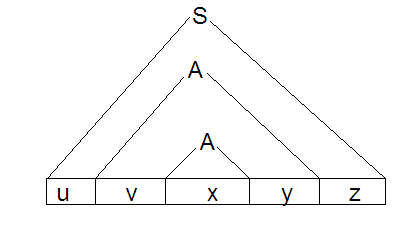
\includegraphics[width=8cm]{assets/13_2_1.png}
\end{center}

Для полного доказательства переходите  \href{https://clck.ru/3LyofA}{сюда}

\hfill Q.E.D.


